\documentclass{article}
\usepackage[utf8]{inputenc}

\usepackage{amsfonts}
\usepackage{amssymb}
\usepackage{amsmath}
\usepackage{amsthm}
\usepackage{enumitem}

\usepackage{bbold}
\usepackage{bm}
\usepackage{graphicx}
\usepackage{color}
\usepackage{hyperref}
\usepackage[margin=2.5cm]{geometry}

\usepackage{float}

\begin{document}


% ==============================================================================

\title{\Large{INFO8006: Project 2 - Report}}
\vspace{1cm}
\author{\small{\bf Maxime Goffart - s180521} \\ \small{\bf Olivier Joris - s182113}}

\maketitle

% ==============================================================================

\section{Problem statement}

\begin{enumerate}[label=\alph*.,leftmargin=*]
    \item
    	\begin{itemize}
    		\item (Initial state) A game state is given by the position of Pacman, the position of the ghost, and the positions of the remaining food dots in the maze.\\
    		The initial state is given by the layout of the maze, the initial position of Pacman, the initial position of the ghost, and the initial positions of all the food dots in the maze.
    		
    		\item (Player function) The player function is a function that takes a state as input and returns a value corresponding to the player who has to play. It respects this principle : an agent takes an action then the other takes one and so on. It is a turn-taking game.
    		
    		\item (Actions) Pacman and the ghost can go north, south, east, or west if they do not go through a wall. Both of them can, also, stay on the same cell.\\
    		If Pacman arrives on a cell with a food, Pacman eats the food.\\
    		If the ghost arrives on the cell where Pacman is, the ghost kills Pacman.
    		
    		\item (Terminal test) True if Pacman has eaten all the foods without being killed or Pacman was killed by the ghost.
    		
    		\item (Transition model) The movement of Pacman or the ghost to another cell will modified their position in the maze under the condition that the movement is legal. If Pacman eats a food, the food is removed from the maze. If the ghost kills Pacman, Pacman is removed from the maze and can no longer play (terminal state).
			
			\item (Utility) Given a game state and a player function, the utility can be described as following : $Utility(s, p) = Game \ score(s)$ where $Game \ score(s)$ is the game score of the actual state $s$.
    	\end{itemize}
    	
    \item Pacman will be the max agent and the ghost will be the min agent. Pacman wants to maximize the utility function (which implies maximizing the game score) by eating all the food dots in a minimum number of time steps without being killed.\\
          The ghost, on its side, wants to kill Pacman as fast as possible to minimize the utility function (which implies minimizing the game score).\\
          This description makes the game of Pacman a zero-sum game because the total payoff to the two players is constant for a given initial layout.
\end{enumerate}

\section{Implementation}

\begin{enumerate}[label=\alph*.,leftmargin=*]
    \item Minimax is complete if the game tree is finite. For the game of Pacman, in general, the game tree is finite because either Pacman will eat all the food dots or the ghost will kill Pacman. However, if the ghost keeps chasing Pacman without being able to kill it and Pacman is not able to eat all the food dots in the meantime, the algorithm will never end.\\
    As for the A$^*$ graph-search algorithm, we could keep a set which will remember the game states already considered so we do not spend computing time to recompute them. This will prevent Pacman and the ghost to do the same movements indefinitely.
    \item \textbf{\textit{Leave empty.}}
    \item \textbf{\textit{Leave empty.}}
	\item Each cutoff-test includes a condition to check whether the game is finished (in a winning or losing end).
		\begin{itemize}
			\item The cutoff-test/evaluation pair implemented in \texttt{hminimax0.py} is :
				\begin{itemize}
					\item Cutoff-test function: $depth \geq 4$
					\item Evaluation function : $score \ - \ pacmanClosestFoodDistance \ - \ 3 \ * \ numFoodsLeft \ - \ 1 \ / \ pacmanGhostDistance$\\
					
					In these functions, for a given state, \textit{pacmanClosestFoodDistance} represents the Manhattan distance between Pacman and the food dot which is the closest to him, \textit{depth} represents the explored depth of the game tree, \textit{score} represents the score of the game state, \textit{numFoodsLeft} represents the number of remaining food dots, and \textit{pacmanGhostDistance} represents the Manhattan distance between Pacman and the ghost.\\
					
					This cutoff-test/evaluation pair allows to cut the exploration at a certain explored depth (fixed here at 4) of the game tree. This pair allows us to evaluate a state in this way : the higher score, the better, the closest Pacman to a food dot is, the better, the less food dots, the better, and the farthest Pacman is from the ghost, the better. The evaluation function is a linear combination of these characteristics allowing to choose a certain weight for each of them as a coefficient.\\
				\end{itemize}

			\item The cutoff-test/evaluation pair implemented in \texttt{hminimax1.py} is :
				\begin{itemize}
					\item Cutoff-test function: $depth \geq 4$
					\item Evaluation function : $10 \ * \ initNumFoods - \ 13 \ * \ numFoodsLeft \ - \ pacmanClosestFoodDistance - \ 1 \ / \ pacmanGhostDistance \ + \ (500 \ if \ winning \ end) \ + \ (-500 \ if \ losing \ end)$ \\
				
					In these functions, for a given state, the names of the features represent the same as in the first pairs of functions. \textit{initNumFoods} represents the initial number of foods in the maze, \textit{winning end} is a condition on whether the game ends in a winning state for Pacman, and \textit{losing end} is a condition on whether the game ends in a losing state for Pacman.\\
				
					This cutoff-test/evaluation pair allows to cut the exploration of the game tree at a certain explored depth (fixed here at 4) of the game tree. The evaluation function is based onto the first one but does not take into account the number of time steps neither the elements of the game score that will always be 0 in this version of the game (the number of eaten capsules and the number of eaten ghosts).\\
				\end{itemize}
				
		\item The cutoff-test/evaluation pair implemented in \texttt{hminimax2.py} is :
				\begin{itemize}
					\item Cutoff-test function: $pacmanGhostDistance \geq pacmanClosestFoodDistance \ or \ depth \geq 4$
					\item Evaluation function : $score \ - \ pacmanClosestFoodDistance \ - \ 3 \ * \ numFoodsLeft \ - \ 1 \ / \ pacmanGhostDistance$\\
				
					In these functions, for a given state, the names of the features represent the same as in the first pair of functions.\\
				
					This cutoff-test/evaluation pair allows to cut the exploration of the game tree when Pacman is closer to the nearest food dot to him than he is from the ghost or at a certain explored depth (fixed here at 4 which is sufficient for the given layouts) of the game tree. This additional condition is used to make sure that the hminimax algorithm get cut at a sufficiently early moment. The evaluation function is the same as the first one.\\
				\end{itemize}
				
		\end{itemize}
\end{enumerate}

\section{Experiment}
a.
	i) Comparison of the scores:
		\begin{figure}[H]
			\centering
			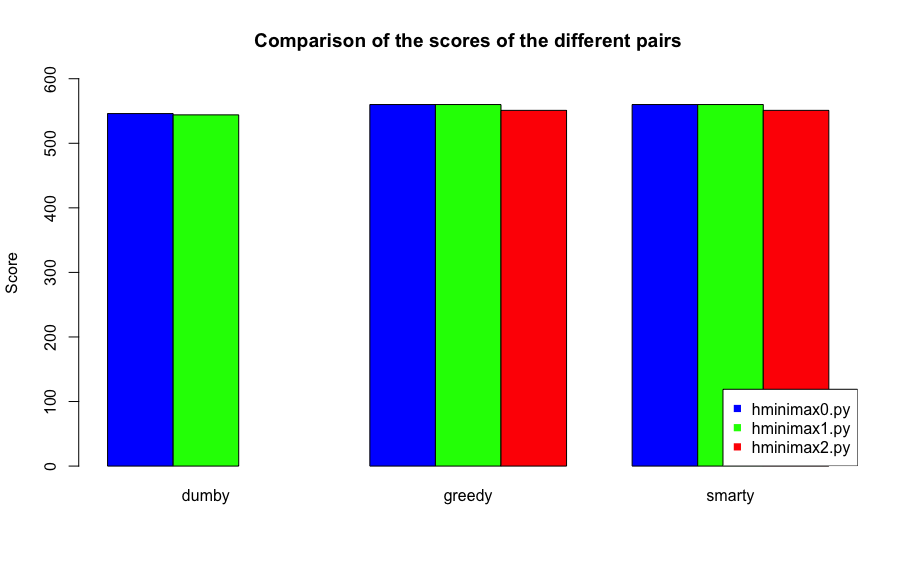
\includegraphics[scale=0.45]{plots/3a_scores.png}
			\caption{Scores of the different cutoff-test/eval pairs in the large layout.}
		\end{figure}
	ii) Comparison of the number of expanded nodes:
		\begin{figure}[H]
			\centering
			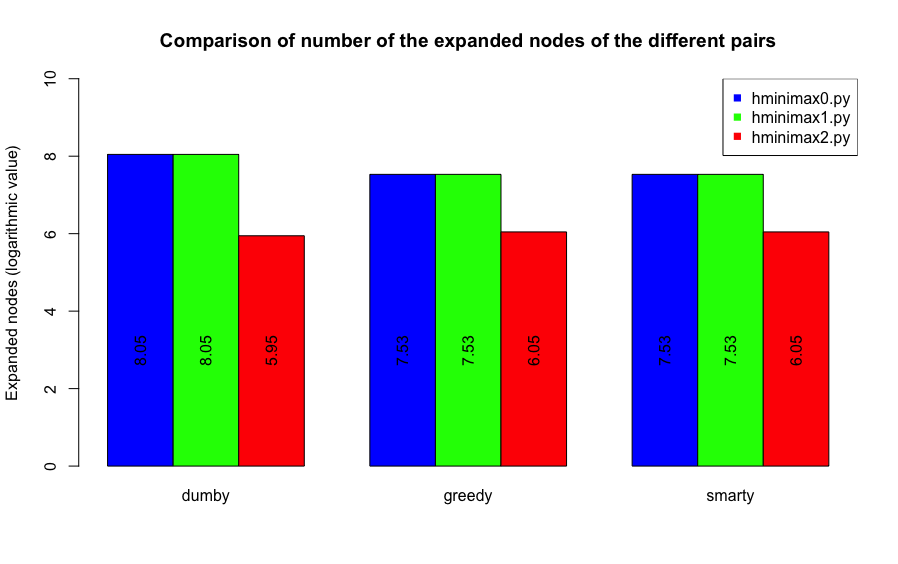
\includegraphics[scale=0.45]{plots/3a_nodes.png} 
			\caption{Number of expanded nodes of the different cutoff-test/eval pairs in the large layout.}
		\end{figure}
	iii) Comparison of the computation times:
		\begin{figure}[H]
			\centering
			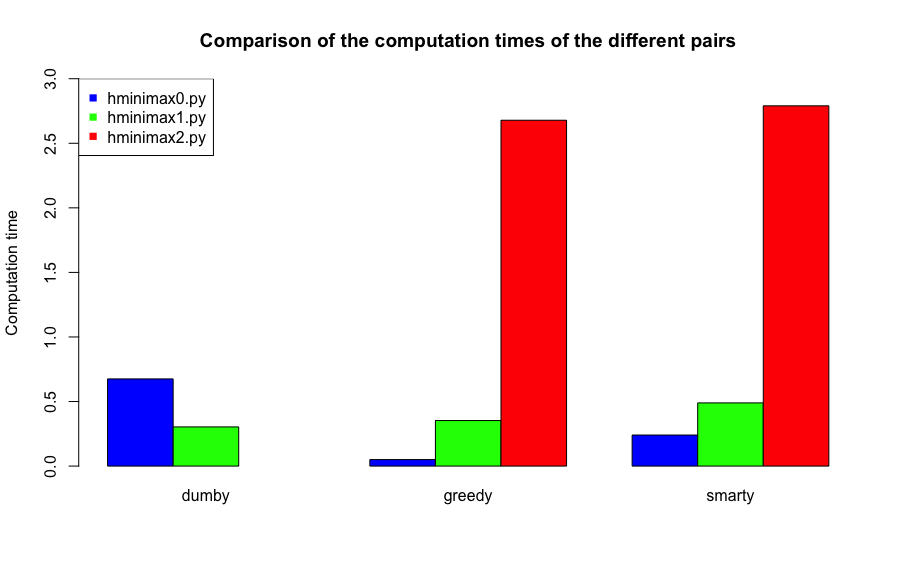
\includegraphics[scale=0.45]{plots/3a_times.png} 
			\caption{Computation times of the different cutoff-test/eval pairs in the large layout.}
		\end{figure}
\begin{enumerate}[label=\alph*.,leftmargin=*]	
	\item[b.] All the cutoff-test/evaluation pairs allow Pacman to win against all the ghosts in the provided layouts.\\
	The first 2 cutoff-test/evaluation pairs give the same scores with the same number of expanded nodes. The first pair does it in the same time or slightly faster than the second pair.\\
	The third pair provides scores that are slightly higher than the ones of the first 2 pairs. The small differences can be explained by the fact that the cut-off is more sophisticated. However, it always takes way less time and a fraction of the number of expanded nodes. Despite this, we consider this pair as our least one because it may lead to the death of Pacman for certain layouts on which Pacman is able to win.

    \item[c.] To handle several ghosts, we need to label states with utility tuples (1 value per agent). Each agent will now want to maximize its own value, it can give rise to cooperation between agents (in this game, all the ghosts want to kill Pacman). The game can no longer be described as a zero-sum game because the total payoff to all players is no longer constant.

\end{enumerate}

% ==============================================================================

\end{document}